\chapter{[Właściwy dla kierunku - np.Specyfikacja wewnętrzna]}
Jeśli to Specyfikacja wewnętrzna:
\begin{itemize}
\item przedstawienie idei
\item architektura systemu
\item opis struktur danych (i organizacji baz danych)
\item komponenty, moduły, biblioteki, przegląd ważniejszych klas (jeśli występują)
\item przegląd ważniejszych algorytmów (jeśli występują)
\item szczegóły implementacji wybranych fragmentów, zastosowane wzorce projektowe
\item diagramy UML
\end{itemize}


\begin{itemize}
    \item wymagania funkcjonalne i niefunkcjonalne
    \item przypadki użycia (diagramy UML) - dla prac, w których mają zastosowanie
    \item opis narzędzi, metod eksperymentalnych, metod modelowania itp.
    \item metodyka pracy nad projektowaniem i implementacją - dla prac, w których ma to zastosowanie
    \end{itemize}
    
    \section{Rozpoznawanie dłoni}
    
    \quad Pierwszym elementem projektu jest rozpoznanie dłoni poprzez wyznacznie pozycji elementów charakterystycznych. Pozycja każdego z tych elementów jest względna wedłgu pozycji nadgarstka. ????
    
    
    %%%%%%%%%%%%%%%%%%%%%%%%%%%%%%%%%%%%%%%%%%%%%%%%%%%%%%%%%%%%%%%%%%%%
    %%%%%%%%%%%%%%%%%%%%%%%%%%%%%% OPEN CV %%%%%%%%%%%%%%%%%%%%%%%%%%%%%
    %%%%%%%%%%%%%%%%%%%%%%%%%%%%%%%%%%%%%%%%%%%%%%%%%%%%%%%%%%%%%%%%%%%%
    \subsection{OpenCV - przygotowanie obrazu z kamery}
    
    \quad Poprawne działanie modelu MediaPipe wymaga odpowiedniego przygotowania obrazu kamery. Działanie kontrolerolera odbywa się poprzez główną metodę \textbf{main()}.
    
    Metoda \textbf{main()} jest główną funkcją, w której dokonywane są obliczenia oraz przeszktałcenia pozwalające na obliczenie obrotu dłonie, odległości między wybranymi palcami oraz na wykrycie gestu. 
    
    % \inputminted[firstline=51, lastline=52]{python}{../OpenLeap.py}
    
    \lstinputlisting[language=python, firstline=51, lastline=52]{../OpenLeap.py}
    
    \quad W pierwszym kroku tworzymy instancję klasy \textbf{VideoCapture} biblioteki \textbf{OpenCV}, która pozwoli na odczytywanie obrazu kamery. 
    
    \lstinputlisting[language=python, firstline=272, lastline=297]{../OpenLeap.py}
    
    % \inputminted[firstline=272, lastline=297]{python}{../OpenLeap.py}
    
    %%%%%%%%%%%%%%%%%%%%%%%%%%%%%%%%%%%%%%%%%%%%%%%%%%%%%%%%%%%%%%%%%%%%
    %%%%%%%%%%%%%%%%%%%%%%%%%%%% MEDIA PIPE %%%%%%%%%%%%%%%%%%%%%%%%%%%%
    %%%%%%%%%%%%%%%%%%%%%%%%%%%%%%%%%%%%%%%%%%%%%%%%%%%%%%%%%%%%%%%%%%%%
    
    \subsection{MediaPipe - Elementy charakterystyczne}
    
    \quad Biblioteka MediaPipe o otwartym źródle, udostępnia wieloplatformowe oraz konfigurowalne rozwiązania wykrzustujące uczenie maszynowe w dziedzienie rozpoznawania, segmentacji oraz klasyfikacji obiektów wizji komputerowej. Niektórymi z rozwiązań są:
    
    \begin{itemize}
        \item Rozpoznawanie twarzy
        \item Segmentacjia włosów oraz twarzy
        \item Rozpoznawnie oraz określanie rozmiarów obiektów trójwymiarowych 
              na podstawie obrazu dwuwymiarowego. 
    \end{itemize}
    
    \quad Model modułu MediaPipe pozwala na wyznaczenie pozycji 21 elementów charakterystycznych dłoni. Współrzędne X i Y są znomralizowane względem rozdzielczości obrazu kamery. Współrzędna X względem liczby pikseli w osi X, a współrzędna Y względem liczby pikseli w osi Y. Oś Z jest prostopadła do osi X i Y, z punktem początkowym w punkcie określającym pozycję nadgarstka. Współrzędna Z jest znormalizowana względem szerokości obrazu kamery, tak jak współrzędna X. 
    
    \begin{figure}[H]
    \begin{center}
        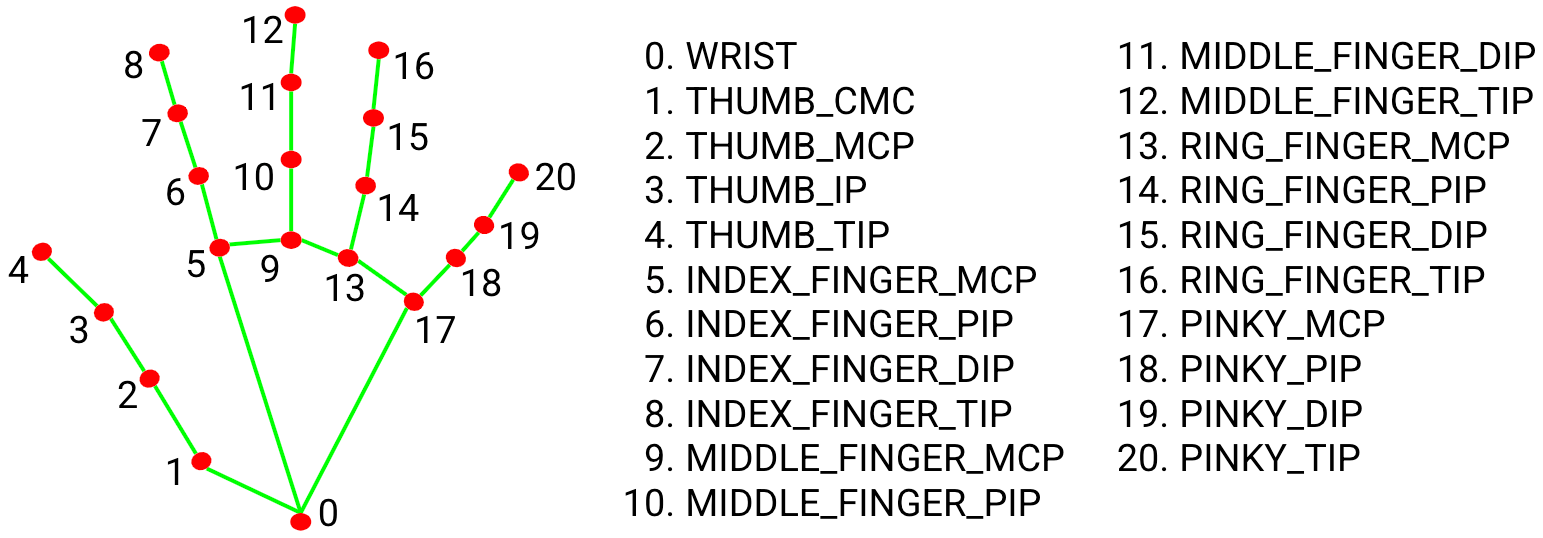
\includegraphics[width=15cm]{../images/hand_landmarks.png}
        \caption{Elementy charakterystyczne dłoni}
    \end{center}
    \end{figure}
    
    \quad Pozycje nadgarstka, paliczków oraz stawów dłoni zostaną wykorzystane do obliczenia obrotu dłoni względem punkut 0 oraz do wytrenowania modeli uczenia maszynowego, których zadaniem będzie rozpoznawnie wybranych gestów. 
    
    \subsection{Generowanie grafiki dłoni}
    
    \quad Generowanie grafiki nałożonej na daną dłoń wykonuje się przy pomocy przygotowanej funkcji biblioteki MediaPipe, która współpracuje z OpenCV. 
    
    %%%%%%%%%%%%%%%%%%%%%%%%%%%%%%%%%%%%%%%%%%%%%%%%%%%%%%%%%%%%%%%%%%%%
    %%%%%%%%%%%%%%%%%%%%%%%%%%% SciKit Learn %%%%%%%%%%%%%%%%%%%%%%%%%%%
    %%%%%%%%%%%%%%%%%%%%%%%%%%%%%%%%%%%%%%%%%%%%%%%%%%%%%%%%%%%%%%%%%%%%
    
    
    \section{SciKit Learn - uczenie maszynowe}
    
    \quad SciKit Learn to biblioteka, która oferuje różnego typu metody uczenia maszynowego. Biblioteka zawiera algorytmy klasyfikacji, regresjii oraz analizy skupień. Przykładowym algorytmami w bibliotece są:
    
    \begin{itemize}
        \item Las losowy - polegająca na konstruowaniu wielu drzew decyzyjnych w czasie uczenia. 
        \item Algorytm centroidów - algorytm wykorzystywany w analizie skupień.
        \item Maszyna wektorów nośnoych - algorytm klasyfikujący, często wykorzystywany w procesie rozpoznawania obrazów. 
    \end{itemize}
    
    O wszystkich dostępnych algorytmach informacje można znaleźć w ogólnodostępnej dokumentacji biblioteki. 
    
    
    
    \subsection{Budowa programu}
    Celem programu będzie stworzenie modeli matematycznych przy pomocy metod uczenia maszynowego, których celem będzie rozpoznawanie gestów dłoni. Proces tworzenie takiego modelu można podzielić na trzy kroki.
    
    \begin{itemize}
        \item Zebranie i przetworzenie danych. 
        \item Przygotowanie algorytmów klasyfikacji i znalezenie najdokładniejszego. 
        \item Zapis modelu do pliku typu \textbf{pickle}
    \end{itemize}
    
    \subsection{Zebranie danych}
    
    \quad Przygotowanie danych do przetworzenia będzie wymagało paru opercaji matematycznych. Współrzędne opisujące pozycje elementów charakterystycznych są znormalizowane względem wielkości obrazu pobranego z kamery, z czego wynika, że środek układu współrzęnych jest w prawym górnym rogu obrazu pobranego z kamery. W takim wypadku należy przprowadzić transformację, tutaj akurat przesunięcie układu współrzędnych do pozycji nadgarstka. Taka operacja pozwoli na pozbycie się uniezależnienie zmiennych od pozycji elementów dłoni na obrazie. Ostatecznie pozbywamy się pozycji nadarstka z wektora danych, ponieważ jest ona środkiem nowego układu współrzędnych. 
    
    \quad \textbf{Macierz przesunięcia}
    
    \begin{equation*}
        M_p = 
        \begin{bmatrix}
        1 & 0 & 0 & -x_0 \\
        0 & 1 & 0 & -y_0 \\
        0 & 0 & 1 & -z_0 \\
        0 & 0 & 0 & 1
        \end{bmatrix}
    \end{equation*}
    
    \quad Aby dane mogły zostać zinterpretowane przez algorytmy ucznenia maszynowego muszą one zostać przedstawione w postaci jednowymiarowej. Aktualna postać macierzy przedstawiającej wpółrzędne elementów charakterystycznych ma następującą postać. Indeksy współrzędnych są równoznaczne z indeksami elementów dłoni. 
    
    \begin{equation*}
        M_p = 
        \begin{bmatrix}
        x_1' & y_1' & z_1' \\
        x_2' & y_2' & z_2' \\
         & \vdots &     \\
        x_{21}' & y_{21}' & z_{21}'
        \end{bmatrix}
    \end{equation*}
    
    Dane w postaci jednowymiarowej mają postać następującego wektora. 
    
    \begin{equation*}
        A_f=
        \begin{bmatrix}
            x_1 & y_1 & z_1 & x_2 & y_2 & \cdots & y_{21} & z_{21}
        \end{bmatrix}
    \end{equation*}
    
    
    \quad Drugim krokiem jest uniezależnienie pozycji elementów od odległości dłoni od kamery. Najprostszym rozwiązaniem jest normalizacja wektora danych względem największej bezwzględnej wartości. 
    
    \quad \textbf{Normalizacja}
    
    % \begin{equation*}
    %     A_n=
        % \begin{bmatrix}
        %     x_1 & y_1 & z_1 & x_2 & y_2 & \cdots & y_{21} & z_{21}
        % \end{bmatrix}
    % \end{equation*}
    
    
    \begin{equation*}
        A_n=\dfrac{A_f}{max(abs(A_f))}
    \end{equation*}
    
    \quad Każdy nowy wektor zostaje zapisany do pliku CSV z odpwowiednią etykietą. Zebrane dane posłużą do wytrenowania algorytmów uczenia maszynowego. 
    
    
    
    \subsection{Metody klasyfikacji - uczenie maszynowe}
    
    \quad Przygotowane dane zostają odczytane z pliku CSV. W pierwszym kroku należy rozdzielić je na dwie części: współrzędne (dane wejściowe) oraz etykiety (dane wyjściowe). W kolejnym kroku należy te dwie grupy podzielić na grupę trenującą i grupę testową. Zadaniem grupy testowej będzie trenowanie wybranych modeli matematycznych, a grupy testowej przetestowanie ich dokładności. 
    
    \quad W celu wybrania najlepszej metody klasyfikacji, zostnie wybranych kilka algorytmów. Każdy z nich stworzy swój model, a ostatecznie zostanie sprawdzona ich poprawności z wykorzystaniem grupy testowej. Model z najepszym wynikiem zostanie zapisany do pliku typu \textbf{pickle}. W języku Python pliki typu \textbf{pickle} pozwalają na zapis zmiennych, obiektów lub innych struktur danych, które mają zostać wykorzystane w po zakończeniu programu. 
    
    \subsection{Ponowne wykorzystanie modelu}
    
    \quad Gotowy model pobieramy i testujemy w przykładowym programie. 
    
    \section{Paczka PyPi}
    \subsection{Budowa paczki}
    
    \quad Ostatecznym krokiem jest przygotowanie programu w formie paczki, która zostanie udostępniona na platformie PyPi. Wygama to przygotowania odpowiednich plików konfiguracyjnych oraz zostosowania stosownych narzędzi do stworznie pliku \textbf{wheel} oraz \textbf{tar}. 
    
    \subsection{Struktura Paczki}
    \quad Pierwszm krokiem jest przygotowanie odpowiedniej struktury paczki. Do tego celu został stworzony folder o poniższej strukturze. W tym folderze znajdują się wszystkie potrzebne elementy paczki. W podfolderze o tej samej nazwie znajduje się główna części modułu, czyli plik .py, w którym zapisana jest klasa OpenLeap. Dodatkowo w tym folderze znajdują się pliki typu \textbf{pickle}, w których zapisane są modele rozpoznające gesty.
    
    \begin{figure}
    \centering
        \begin{minipage}{7cm}
            \dirtree{%
            .1 openleap.
            .2 openleap.
            .3 \hyperref[openleap-file1]{\_\_init\_\_.py}.
            .3 \hyperref[openleap-file2]{OpenLeap.py}.
            .3 \hyperref[openleap-file3]{gesture\_recognition.pkl}.
            .3 \hyperref[openleap-file4]{sign\_language\_alphabet.pkl}.
            .2 LICENSE.
            .2 MANIFEST.
            .2 README.md.
            .2 setup.py.
            } 
        \end{minipage}
        \caption{Struktura paczki PyPi}
    \end{figure}
    
    \subsection{Pliki Konfiguracyjne}
    \quad Pliki setup.py oraz MANIFEST są plikami, które odpowiadają za konfigurację oraz opis paczki. W pliku setup.py zapisany jest numer aktualnej wersji, autor, kontakt do autora, nazwa paczki itp. 
    
    \quad 
    
    
    % \subsection{Plik setup.py}
    \subsection{Załadowanie paczki do repozytorium}
    
    \quad Przed załadowaniem paczki do repozytorium, należy stworzyć zapakowaną paczkę źródłową, na przykład typu .tar oraz plik typu WHEEL. Oba pliki spełniają tą samą funkcję, czyli przechowywnie niezbędnych elementów paczki oraz umożliwiają ich instalację na systemie użytkownika. Plik WHEEL pozwala na dużo szybszy proces instalacji niż instalacja ze źródła, czyli paczki typu .tar. 
